% Options for packages loaded elsewhere
\PassOptionsToPackage{unicode}{hyperref}
\PassOptionsToPackage{hyphens}{url}
\PassOptionsToPackage{dvipsnames,svgnames,x11names}{xcolor}
%
\documentclass[
  a4paper,
]{scrreport}

\usepackage{amsmath,amssymb}
\usepackage{iftex}
\ifPDFTeX
  \usepackage[T1]{fontenc}
  \usepackage[utf8]{inputenc}
  \usepackage{textcomp} % provide euro and other symbols
\else % if luatex or xetex
  \usepackage{unicode-math}
  \defaultfontfeatures{Scale=MatchLowercase}
  \defaultfontfeatures[\rmfamily]{Ligatures=TeX,Scale=1}
\fi
\usepackage{lmodern}
\ifPDFTeX\else  
    % xetex/luatex font selection
\fi
% Use upquote if available, for straight quotes in verbatim environments
\IfFileExists{upquote.sty}{\usepackage{upquote}}{}
\IfFileExists{microtype.sty}{% use microtype if available
  \usepackage[]{microtype}
  \UseMicrotypeSet[protrusion]{basicmath} % disable protrusion for tt fonts
}{}
\makeatletter
\@ifundefined{KOMAClassName}{% if non-KOMA class
  \IfFileExists{parskip.sty}{%
    \usepackage{parskip}
  }{% else
    \setlength{\parindent}{0pt}
    \setlength{\parskip}{6pt plus 2pt minus 1pt}}
}{% if KOMA class
  \KOMAoptions{parskip=half}}
\makeatother
\usepackage{xcolor}
\setlength{\emergencystretch}{3em} % prevent overfull lines
\setcounter{secnumdepth}{-\maxdimen} % remove section numbering
% Make \paragraph and \subparagraph free-standing
\ifx\paragraph\undefined\else
  \let\oldparagraph\paragraph
  \renewcommand{\paragraph}[1]{\oldparagraph{#1}\mbox{}}
\fi
\ifx\subparagraph\undefined\else
  \let\oldsubparagraph\subparagraph
  \renewcommand{\subparagraph}[1]{\oldsubparagraph{#1}\mbox{}}
\fi


\providecommand{\tightlist}{%
  \setlength{\itemsep}{0pt}\setlength{\parskip}{0pt}}\usepackage{longtable,booktabs,array}
\usepackage{calc} % for calculating minipage widths
% Correct order of tables after \paragraph or \subparagraph
\usepackage{etoolbox}
\makeatletter
\patchcmd\longtable{\par}{\if@noskipsec\mbox{}\fi\par}{}{}
\makeatother
% Allow footnotes in longtable head/foot
\IfFileExists{footnotehyper.sty}{\usepackage{footnotehyper}}{\usepackage{footnote}}
\makesavenoteenv{longtable}
\usepackage{graphicx}
\makeatletter
\def\maxwidth{\ifdim\Gin@nat@width>\linewidth\linewidth\else\Gin@nat@width\fi}
\def\maxheight{\ifdim\Gin@nat@height>\textheight\textheight\else\Gin@nat@height\fi}
\makeatother
% Scale images if necessary, so that they will not overflow the page
% margins by default, and it is still possible to overwrite the defaults
% using explicit options in \includegraphics[width, height, ...]{}
\setkeys{Gin}{width=\maxwidth,height=\maxheight,keepaspectratio}
% Set default figure placement to htbp
\makeatletter
\def\fps@figure{htbp}
\makeatother

%\newfontfamily\Ubuntu[Mapping=tex-text]{Ubuntu}
\usepackage{pgfplots}
\usetikzlibrary{arrows.meta,arrows}
\usetikzlibrary{angles,quotes}
\pgfplotsset{grid style={dashed,mygray}}
% Colors
\definecolor{myblue}{rgb}{0.067,0.529,0.871}
\definecolor{mypurple}{rgb}{0.859,0.071,0.525}
\definecolor{myred}{rgb}{1.0, 0.13, 0.32}
\definecolor{mygreen}{rgb}{0.01, 0.75, 0.24}
\definecolor{myblack}{gray}{0.1}
\definecolor{mygray}{gray}{0.8}
\newcommand{\NN}{\mathbb{N}}
\newcommand{\ZZ}{\mathbb{Z}}
\newcommand{\QQ}{\mathbb{Q}}
\newcommand{\RR}{\mathbb{R}}
\newcommand{\CC}{\mathbb{C}}
\DeclareMathOperator{\Int}{Int}
\DeclareMathOperator{\Ext}{Ext}
\DeclareMathOperator{\Fr}{Fr}
\DeclareMathOperator{\Adh}{Adh}
\DeclareMathOperator{\Ac}{Ac}
\DeclareMathOperator{\sen}{sen}
\makeatletter
\makeatother
\makeatletter
\makeatother
\makeatletter
\@ifpackageloaded{caption}{}{\usepackage{caption}}
\AtBeginDocument{%
\ifdefined\contentsname
  \renewcommand*\contentsname{Indice de contenidos}
\else
  \newcommand\contentsname{Indice de contenidos}
\fi
\ifdefined\listfigurename
  \renewcommand*\listfigurename{Listado de Figuras}
\else
  \newcommand\listfigurename{Listado de Figuras}
\fi
\ifdefined\listtablename
  \renewcommand*\listtablename{Listado de Tablas}
\else
  \newcommand\listtablename{Listado de Tablas}
\fi
\ifdefined\figurename
  \renewcommand*\figurename{Figura}
\else
  \newcommand\figurename{Figura}
\fi
\ifdefined\tablename
  \renewcommand*\tablename{Tabla}
\else
  \newcommand\tablename{Tabla}
\fi
}
\@ifpackageloaded{float}{}{\usepackage{float}}
\floatstyle{ruled}
\@ifundefined{c@chapter}{\newfloat{codelisting}{h}{lop}}{\newfloat{codelisting}{h}{lop}[chapter]}
\floatname{codelisting}{Listado}
\newcommand*\listoflistings{\listof{codelisting}{Listado de Listados}}
\makeatother
\makeatletter
\@ifpackageloaded{caption}{}{\usepackage{caption}}
\@ifpackageloaded{subcaption}{}{\usepackage{subcaption}}
\makeatother
\makeatletter
\@ifpackageloaded{tcolorbox}{}{\usepackage[skins,breakable]{tcolorbox}}
\makeatother
\makeatletter
\@ifundefined{shadecolor}{\definecolor{shadecolor}{rgb}{.97, .97, .97}}
\makeatother
\makeatletter
\makeatother
\makeatletter
\makeatother
\ifLuaTeX
\usepackage[bidi=basic]{babel}
\else
\usepackage[bidi=default]{babel}
\fi
\babelprovide[main,import]{spanish}
% get rid of language-specific shorthands (see #6817):
\let\LanguageShortHands\languageshorthands
\def\languageshorthands#1{}
\ifLuaTeX
  \usepackage{selnolig}  % disable illegal ligatures
\fi
\IfFileExists{bookmark.sty}{\usepackage{bookmark}}{\usepackage{hyperref}}
\IfFileExists{xurl.sty}{\usepackage{xurl}}{} % add URL line breaks if available
\urlstyle{same} % disable monospaced font for URLs
\hypersetup{
  pdftitle={CONVIVE: Big Data para la ciudad inteligente},
  pdflang={es},
  colorlinks=true,
  linkcolor={blue},
  filecolor={Maroon},
  citecolor={Blue},
  urlcolor={Blue},
  pdfcreator={LaTeX via pandoc}}

\title{CONVIVE: Big Data para la ciudad inteligente}
\author{}
\date{}

\begin{document}
\begin{titlepage}

%\AddToShipoutPicture*{\put(0,0){\includegraphics[scale=0.8]{img/background2}}} % Imagen de fondo, requiere el paquete eso-pic.
\begin{center}
\vspace*{5cm}

\Huge
{\textbf{\textsf{CONVIVE: Big Data para la ciudad inteligente}}}

\vspace{0.5cm}
\LARGE
{\textbf{\textsf{}}}

\vspace{1.5cm}


\includegraphics[width=0.4\textwidth]{../img/logos/proyectos.png}
\end{center}

\vfill

\begin{flushleft}
\begin{tabular}{ll}

\includegraphics[width=0.1\textwidth]{../img/logos/aprendeconalf.png} & \parbox[b]{5cm}{\Large\textsf{}\\ \textsf{asalber@ceu.es} \\ \textsf{https://aprendeconalf.es}}
\end{tabular}
\end{flushleft}
\end{titlepage}\ifdefined\Shaded\renewenvironment{Shaded}{\begin{tcolorbox}[borderline west={3pt}{0pt}{shadecolor}, enhanced, interior hidden, frame hidden, boxrule=0pt, breakable, sharp corners]}{\end{tcolorbox}}\fi

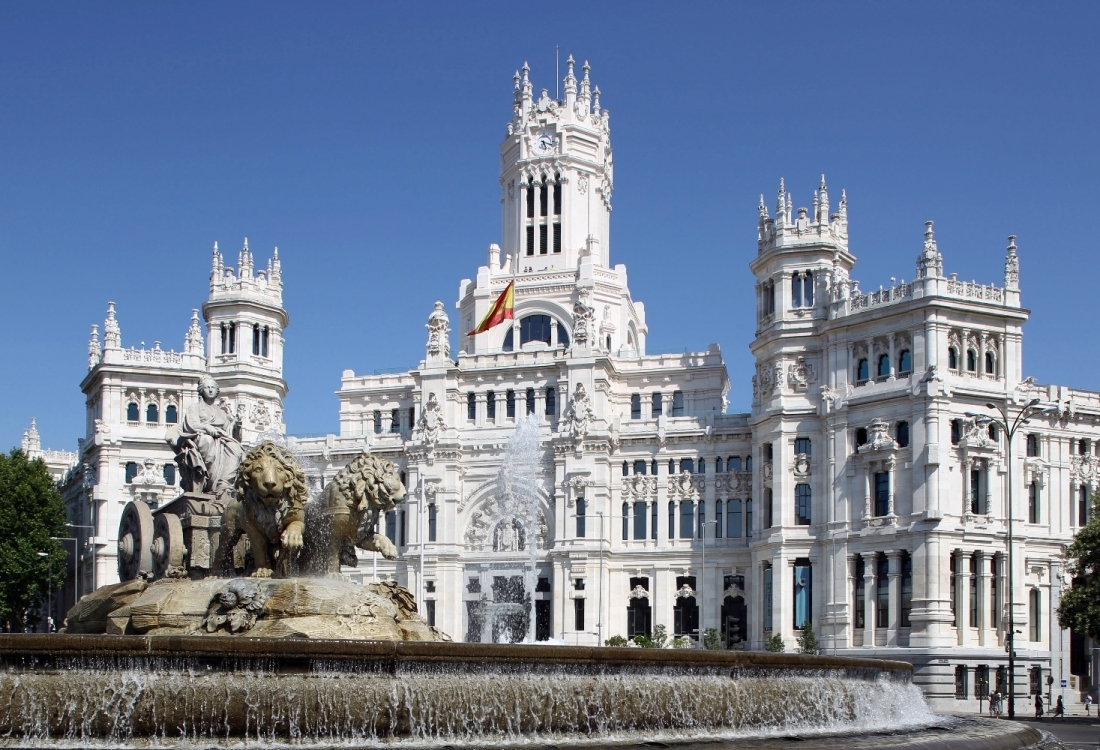
\includegraphics{../img/convive/ayuntamiento-madrid.jpg}

\hypertarget{introducciuxf3n}{%
\section{Introducción}\label{introducciuxf3n}}

Los datos abiertos (open data) es una iniciativa que muchas
administraciones públicas están adoptando con el objetivo de mejorar la
transparencia en lo que respecta a sus funciones de cara a la
ciudadanía.

El ayuntamiento de Madrid es uno de los ayuntamientos que ha empezado a
ofrecer datos en abierto, y en su portal de datos abiertos puede
accederse a multitud de bases de datos con información de todo tipo,
desde los alojamientos en la ciudad hasta las mediciones de
contaminación de las estaciones de registro de contaminantes.

La puesta a disposición de la ciudadanía de toda esta información, no
solo mejora la transparencia sobre la gestión municipal, sino que
permite a ciudadanos o a empresas particulares poder analizar estos
datos para mejorar sus decisiones.

\hypertarget{objetivos}{%
\section{Objetivos}\label{objetivos}}

El objetivo principal del proyecto CONVIVE es mejorar el conocimiento
del estado real de la ciudad a través de la medición de datos de su
entorno y de la información aportada por los ciudadanos. Para ello se
desplegará toda la infraestructura necesaria para adquirir esa
información y tratarla adecuadamente.

Un objetivo específico del proyecto es que el tratamiento de datos debe
realizarse con tecnologías relacionadas con el Big Data. Así nos
aseguraremos de que el sistema pueda integrar fuentes de información
variadas incluso después de que el sistema haya sido creado.

\hypertarget{descripciuxf3n-tuxe9cnica}{%
\section{Descripción técnica}\label{descripciuxf3n-tuxe9cnica}}

El sistema a implementar consiste en una plataforma de análisis de
varias fuentes de información existentes en el Ayuntamiento de Madrid.
Para ello debe solucionar tres aspectos fundamentales:

\begin{enumerate}
\def\labelenumi{\arabic{enumi}.}
\tightlist
\item
  La recogida de información de la ciudad. Este sistema incluye datos de
  dispositivos, de ciudadanos y de entidades.
\item
  La gestión de los datos recogidos. Debe ser lo suficientemente
  genérica para gestionar posibles incertidumbres en los datos propias
  de una ciudad: información incompleta, nuevas fuentes de información,
  nuevos campos en la misma información, etc.
\item
  El análisis de los datos almacenados. Los análisis pueden basarse en
  la combinación de varios conjuntos de datos integrados en el sistema.
  Es necesario tener en cuenta que estos datos pueden estar en
  ubicaciones diferentes y pueden tener un tamaño que no permita su
  adecuado procesamiento en una sola máquina.
\end{enumerate}

En una ciudad el número de fuentes de información no está fijado ya que
en cualquier momento pueden aparecer nuevas fuentes de información a
medida que se implanten tecnologías nuevas o formas distintas de
participar por parte de los ciudadanos. En el proyecto CONVIVE se
definen algunas fuentes de información que deben ser tratadas y se
emplean tecnologías que faciliten la integración de nuevas fuentes de
información en el futuro. Las fuentes de información que debe gestionar
CONVIVE son:

\begin{itemize}
\tightlist
\item
  Avisos de incidencias en la vía pública por parte de los ciudadanos.
  El sistema integrará estos avisos tanto de forma interactiva (para
  gestionar la incidencia) como de forma procesada (registros de avisos
  durante un periodo de tiempo).

  \begin{itemize}
  \tightlist
  \item
    Los avisos interactivos se almacenarán en un sistema que permita la
    actualización del estado de los mismos.
  \item
    Los avisos procesados suelen corresponder a avisos interactivos que
    han sido transformados a un formato que facilita su procesamiento
    estadístico. De esta forma se podrá relacionar estos avisos con
    otras fuentes estadísticas disponibles en la ciudad.
  \end{itemize}
\item
  Información acústica de la ciudad. El sistema integrará los datos del
  nivel de ruido existente en distintas partes de la ciudad. Para ello
  obtendrá la información de ruido en determinadas zonas y los
  registrará para su posterior análisis.
\end{itemize}

Para llevar a cabo el proyecto CONVIVE se divide su desarrollo en tres
subsistemas distintos que coinciden con los tres aspectos a solucionar
previamente comentados.

\hypertarget{subsistema-de-adquisiciuxf3n-de-datos}{%
\subsection{Subsistema de adquisición de
datos}\label{subsistema-de-adquisiciuxf3n-de-datos}}

En este subsistema de deben solucionar aspectos relacionados con la
recogida de la información. Para ello debe desplegar una red de sensores
acústicos en la ciudad (encargados del proceso de recogida de
información de ruido) y habilitar un sistema de comunicación para los
ciudadanos (con el fin de generar avisos de incidencias en la vía
pública).

En el proyecto CONVIVE tendremos dos tipos de información al finalizar
el trabajo en este subsistema:

\begin{enumerate}
\def\labelenumi{\arabic{enumi}.}
\tightlist
\item
  Una base de datos con información sobre las incidencias reportadas por
  los ciudadanos. En esta base de datos se almacenan las incidencias
  activas y cuyo estado se puede actualizar. Como criterio de diseño se
  almacenarán en una base de datos (no en un fichero) ya que tiene
  ciertas ventajas para su gestión.
\item
  Información relacionada con los niveles de ruido. Se recogerá
  información de los sensores desplegados en la ciudad y se almacenarán
  en ficheros con formato CSV.
\end{enumerate}

\begin{figure}

{\centering 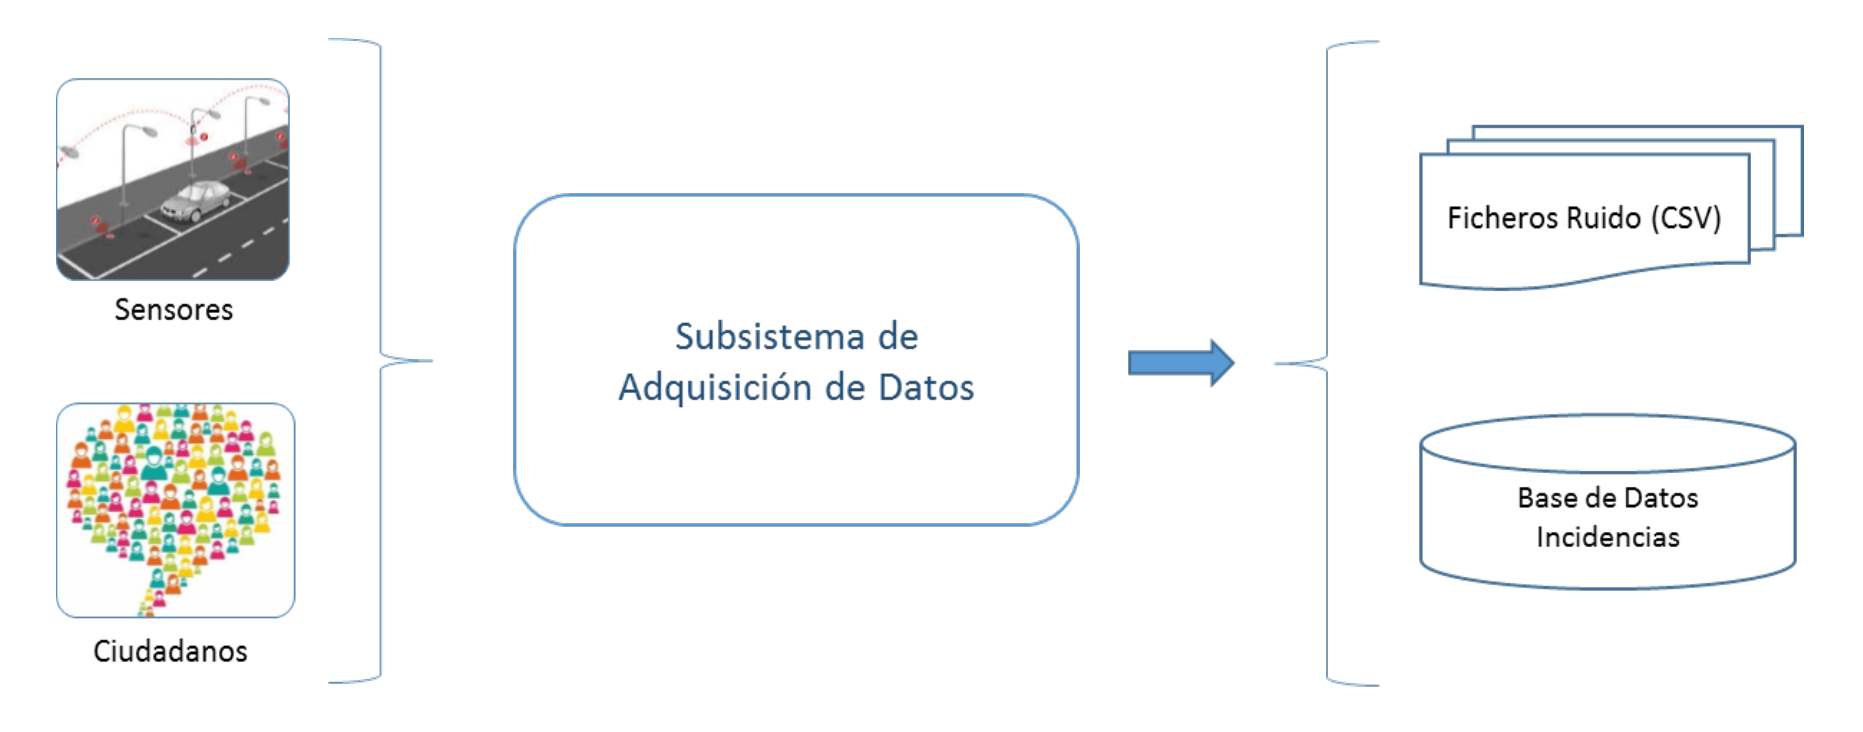
\includegraphics{../img/convive/subsistema-adquisicion-datos.png}

}

\caption{Subsistema de adquisición de datos}

\end{figure}

\hypertarget{subsistema-de-gestiuxf3n-de-datos}{%
\subsection{Subsistema de gestión de
datos}\label{subsistema-de-gestiuxf3n-de-datos}}

En este subsistema de deben solucionar aspectos relacionados con el
almacenamiento y sincronización de la información a través de distintas
máquinas.

Dado que no se implementará realmente el subsistema de adquisición de
datos (aunque sí se llevará a cabo un diseño detallado), se obtendrán
datos del sistema AVISA que contiene las incidencias reportadas por los
ciudadanos, y del nivel de ruidos del Ayuntamiento de Madrid.

Una vez que se disponga de todos los datos como ficheros en formato CSV
(los datos de AVISA y los de ruido) utilizaremos un sistema que permita
distribuirlos a través de varias máquinas y sincronizarlos para
facilitar su acceso.

\begin{figure}

{\centering 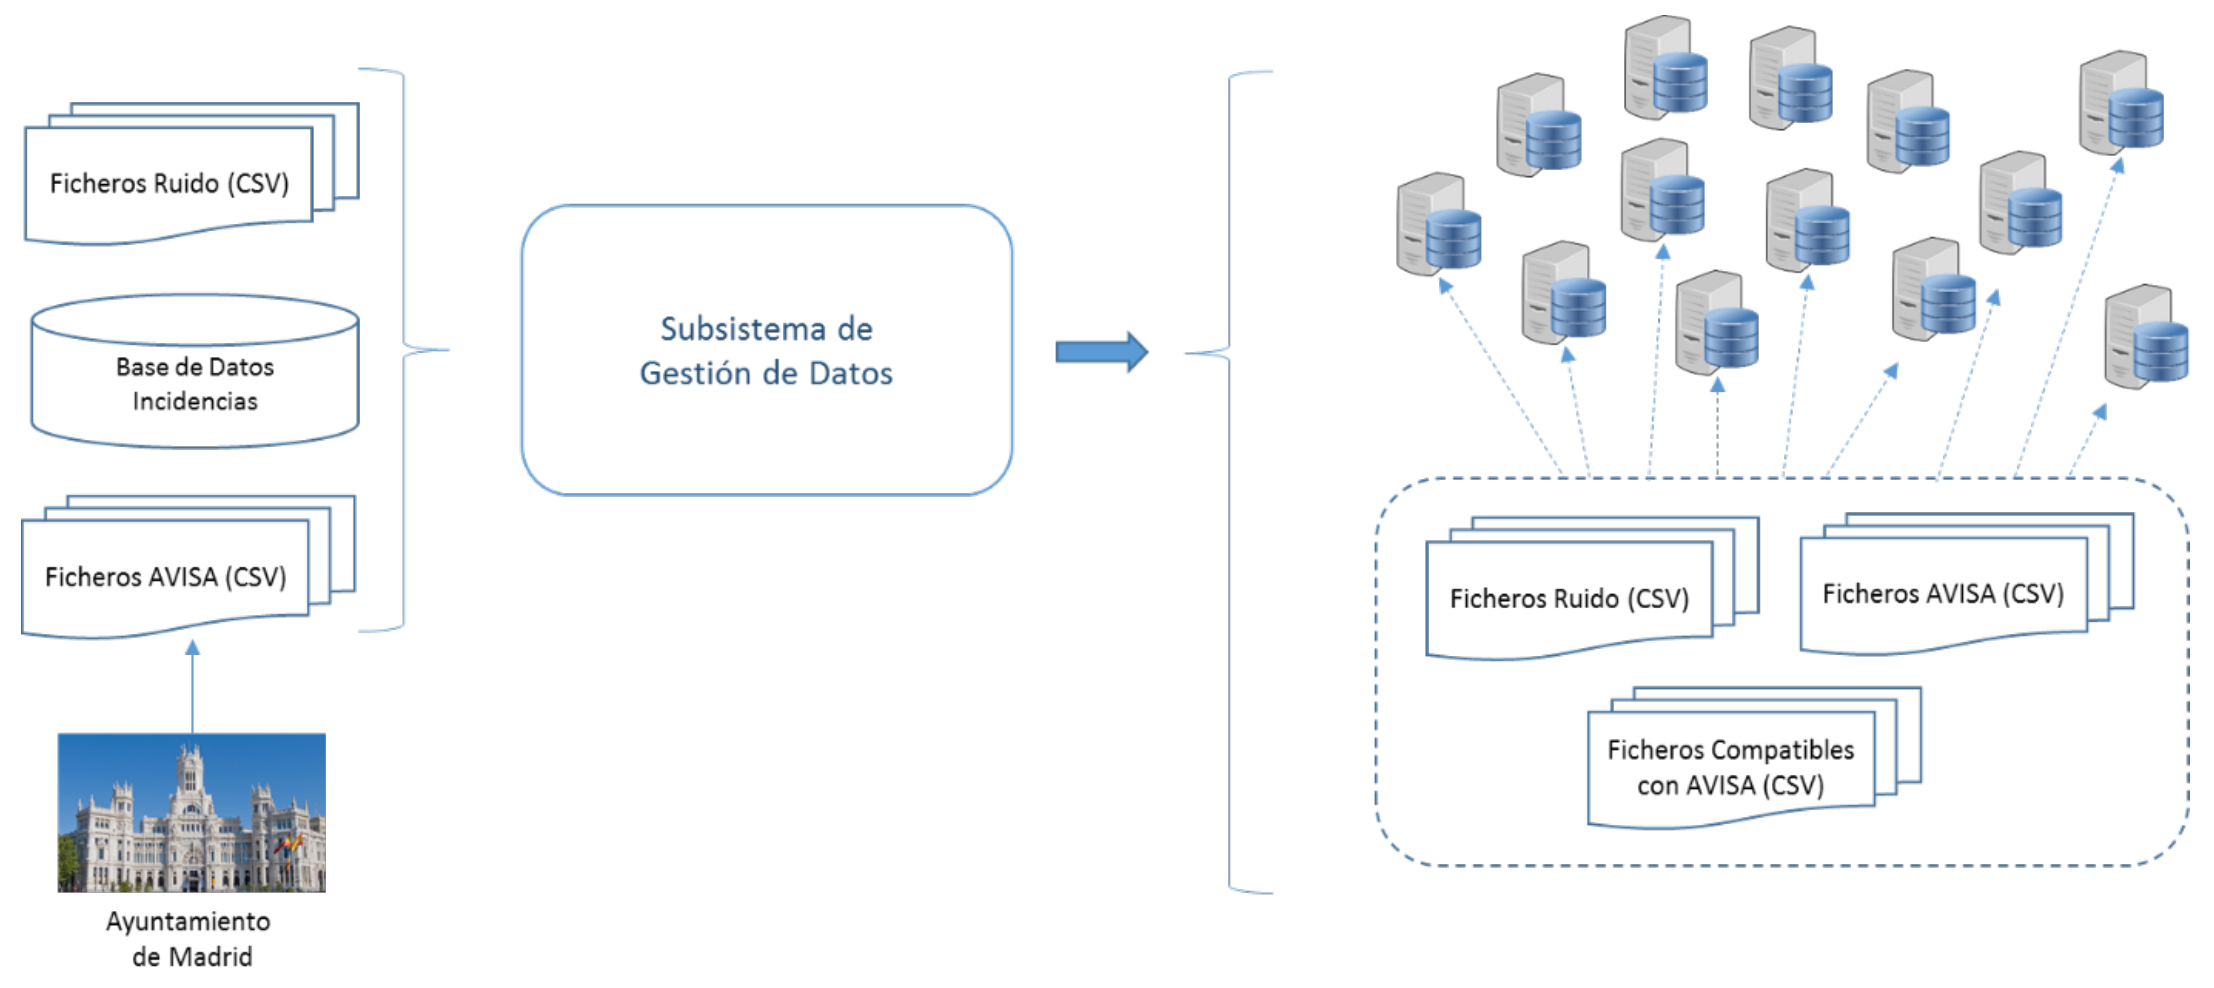
\includegraphics{../img/convive/subsistema-gestion-datos.png}

}

\caption{Subsistema de gestión de datos}

\end{figure}

\hypertarget{subsistema-de-anuxe1lisis-de-datos}{%
\subsection{Subsistema de análisis de
datos}\label{subsistema-de-anuxe1lisis-de-datos}}

En este subsistema se obtiene información útil a partir de todos los
datos disponibles. En un sistema real se cruzarían los datos del sistema
AVISA, con los de niveles de ruido y con varios datos más para obtener
información sintetizada y en muchos casos inferir relaciones entre
distintos hechos que estén ocurriendo. En el caso del proyecto CONVIVE,
por motivos de claridad a la hora de aprender conceptos, se utilizará
únicamente un fichero con los datos del sistema AVISA en formato CSV. Se
descartarán tanto los datos de ruido como cualquier otro tipo de fuente
de datos que puede obtenerse del Ayuntamiento de Madrid.

En el proyecto CONVIVE se realizarán dos acciones con los datos:

\begin{enumerate}
\def\labelenumi{\arabic{enumi}.}
\item
  Se analizarán los datos existentes del sistema AVISA para obtener
  información sintetizada de los incidentes reportados. Para ello debe
  tenerse en cuenta que el fichero con los datos puede estar repartido
  entre varias máquinas y que se debe utilizar un modelo de programación
  que facilite el acceso a todos esos datos sin cargar la máquina en la
  que se ejecute.
\item
  Se visualizarán los datos del sistema AVISA para que sean más
  fácilmente entendibles por los destinatarios finales. Las decisiones
  finales sobre las acciones a tomar las llevarán a cabo por personas
  con distintas capacidades de abstracción y síntesis. Para facilitar
  esas decisiones se mostrarán los datos mediante modelos visuales que
  permitan una mejor comprensión de éstos.
\end{enumerate}

\begin{figure}

{\centering 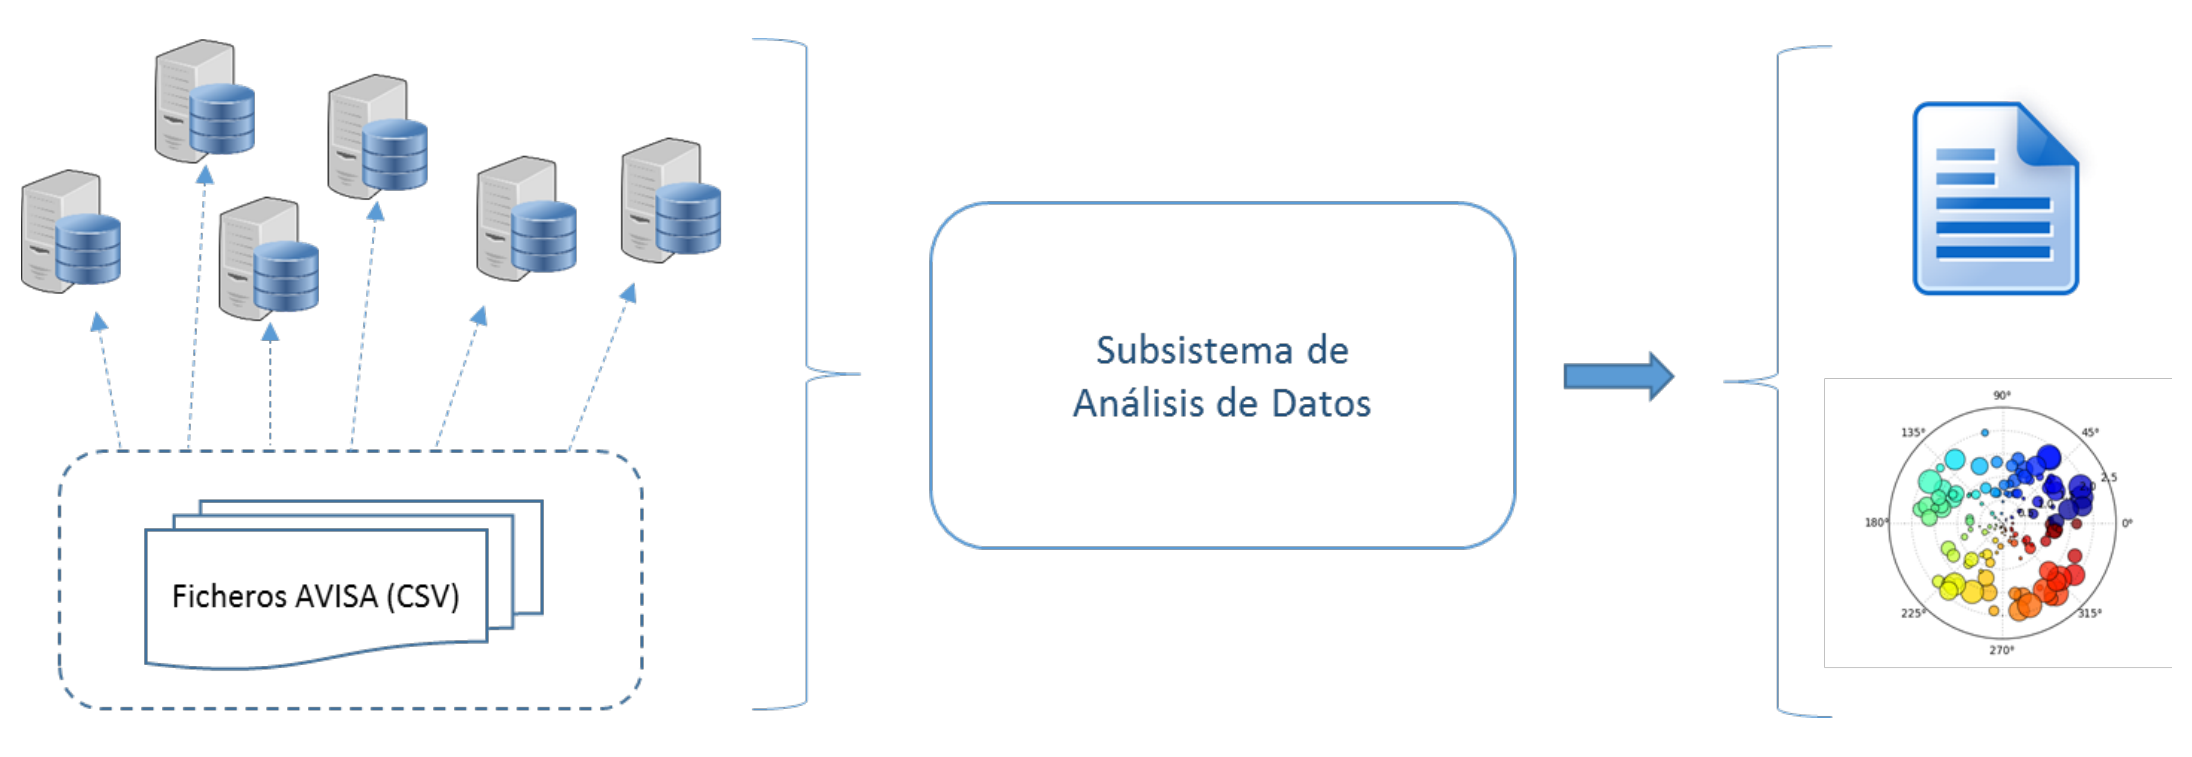
\includegraphics{../img/convive/subsistema-analisis-datos.png}

}

\caption{Subsistema de análisis de datos}

\end{figure}

\hypertarget{tareas}{%
\section{Tareas}\label{tareas}}

\begin{enumerate}
\def\labelenumi{\arabic{enumi}.}
\tightlist
\item
  Obtener los ficheros de datos del sistema AVISA del Ayuntamiento de
  Madrid.
\item
  Obtener los ficheros de ruido del Ayuntamiento de Madrid.
\item
  Crear el procedimiento de transformación de entradas de la base de
  datos en ficheros en formato compatible con los del sistema AVISA.
\item
  Incluir todos los ficheros, los del sistema AVISA, los generados a
  partir de la base de datos y los de ruido, en un sistema de ficheros
  distribuido.
\item
  Preprocesar el conjunto de datos para prepararlo para el análisis
  estadístico.
\item
  Realizar un análisis estadístico de las principales variables
  incluidas en el conjunto de datos.
\item
  Crear gráficos de visualización de los datos correspondientes a las
  principales variables del conjunto de datos.
\end{enumerate}

\hypertarget{datos}{%
\section{Datos}\label{datos}}

Se obtendrán ficheros con información del
\href{http://datos.madrid.es/portal/site/egob}{portal de datos abiertos
del Ayuntamiento de Madrid}. Este portal tiene un catálogo de datos
disponibles bajo los principios de la iniciativa Datos Abiertos (Open
Data), que impulsa la publicación abierta, regular, reutilizable y
autorizada de los datos de carácter público. En concreto se utilizarán
los conjuntos de datos siguientes:

\begin{itemize}
\tightlist
\item
  Datos del Sistema AVISA. Tiene información de avisos de ciudadanos
  sobre incidencias en la vía pública. Es un fichero en formato CSV.
\item
  Información de la contaminación acústica. Es otro fichero en formato
  CSV.
\end{itemize}



\end{document}
